\documentclass{article}
\twocolumn
\usepackage[T1]{fontenc}
\usepackage{amsmath}
\usepackage[a4paper, total={7in, 9in}]{geometry}
\usepackage{graphicx}
\graphicspath{ {./SS/} }

\begin{document}

\subsubsection*{Komodo Dragon Background Information}
\begin{itemize}
    \item largest reptile
    \item poisonous because it eats alot of rotten food and there is poisonous bacteria present in its saliva which can be paralyzing if you are hit.
    \item sexy ang mga brown
    \item example: there is a female komodo dragon thats attracted to a brown komodo dragon. The tail will hit the female komodo dragon until the dragon is tired and will then have the penis inserted.
    \item Gold/Yellow Komodo Dragons are indications that they're pregnant
    \item The Komodo Dragons then got pregnant without the need of a male
    \item Theres more female Komodo Dragons now
    \item parthenogenesis, two eggs fusing in komodo Dragons
    \item it happens in lizards
    \item Komodo moving tail, and then male realizes the female is in heat, and will then beat the female one and then sex
    \item Are the cells that are birthed from the two eggs fusing the same as the one of the mother?
\end{itemize}

\section*{The Concept of Genes}
\subsubsection*{What are genes?}
\begin{itemize}
    \item Canis familiaris (dogs) have the same set of genes, and in theory as long as they are dogs they can breed?
    \item This is due to them having the same set of genes, but have high variations, so their sex cells can still breed.
\end{itemize}
\subsubsection*{What makes up the chromosomes?}
\includegraphics[scale=1]{dns.png}
\begin{itemize}
    \item Recall: DNA can be used as a blueprint of RNA, which is the blueprint for proteins which make up our body. Any particular change in the DNA leads to variations in the proteins which is why it is important to the identity of an organism.
    \item DNA: The identity of the chromosomes
    \item Histones: They arrange the DNA into clumps which are known as nucleosomes
    \item Nucleosomes: They're brought together to make a coil
    \item Coils: Turn into Supercoils
    \item Supercoils: Turn into Chromosomes with a butterfly shape
    \item Chromosome: Does not always have the butterfly shape, but is only when it is about to divide.
    \item Chromosome number: equation, 2n = 46 for humans
    \item Chromatid: What the DNA should be called if it is not condensed; there are two in a Chromosome, and are identical to each other.
    \item Chromatin: DNA and histones not binded
    \item Telomere, the end of the chromatids
\end{itemize}
\subsubsection*{Centromere and Kinetochore}
Centromere



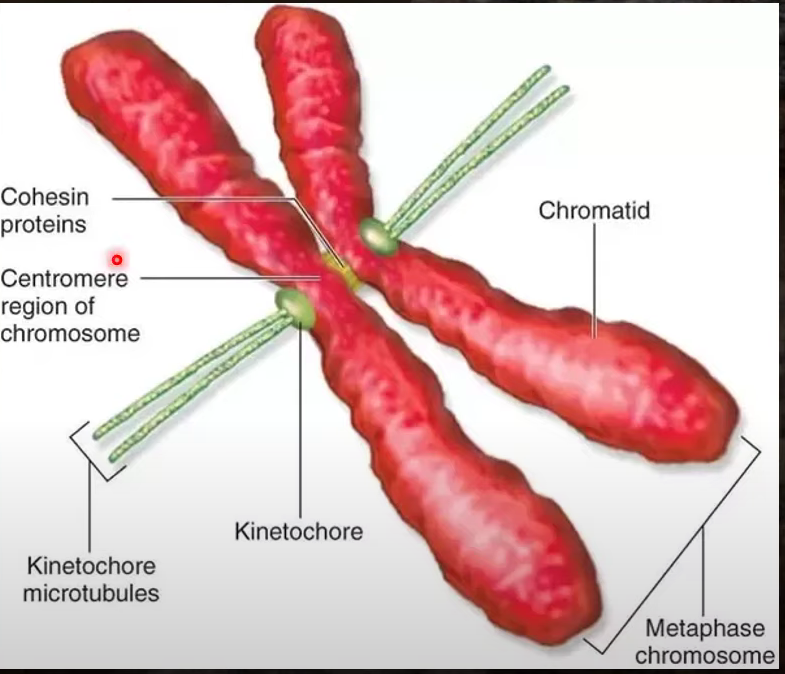
\includegraphics[scale=0.6]{centromere.png}
\begin{itemize}
    \item Does not have to be at the middle, and can be found at any part of the chromatids
    \item Centre of the chromosome that are joined (think of it was the linked area)
\end{itemize}
Kinetochore



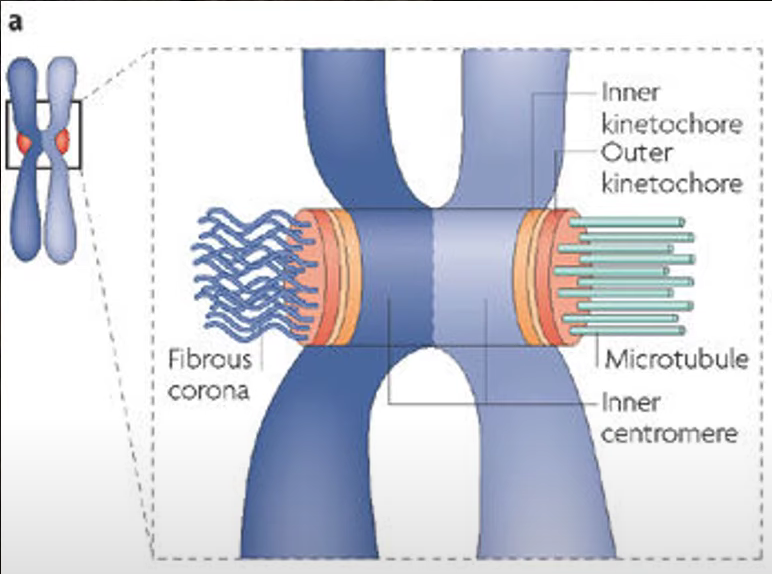
\includegraphics[scale=0.3]{kinetochore.png}
\begin{itemize}
    \item Proteins that can be found in the Centromere region
    \item Serves as an anchor for the chromatids so it can be separated properly without damaging the chromatids.
    \item The Kinetochore walks along the spindle fiber
    \item Recall: The vacuoles have motor proteins guided by the microtubules
    \item Kinetochore uses microtubules/spindle fibers to be guided to the opposite poles to the cells
    \item These microtubules are called Kinetochore microtubules
    \item Kinetochore microtubules provide this path for the Kinetochore, so it would be clear between the two chromatids.
\end{itemize}
Cohesive proteins
\begin{itemize}
    \item Is between the two chromatids
\end{itemize}
\subsubsection*{Genes, Alleles, Locus, Homologous Pairs}
We always have a pair for one chromosomes, there is a paternal and a maternal pair.
\subsubsection*{Homologous Pairs}
\begin{itemize}
    \item They have the same size
    \item In a particular locus you can find the particular gene.
    \item Locus would be the address of the gene, where you find the variation.
    \item The allele is what the variation is called.
\end{itemize}
\subsubsection*{Counting of Chromosome numbers (refer to figure below)}
\begin{itemize}
    \item Starts at 2n = 2
    \item Mother would have 2n = 2, and the father would have 2n = 2
    \item Offspring is 2n = 2 as only 1 side of the pair is taken for the offspring, so it is still 2n = 2, 
    \item For a homologue there is two chromatids
\end{itemize}
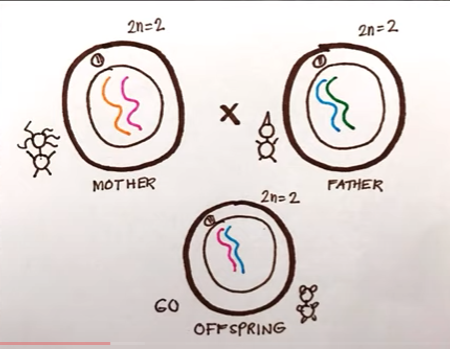
\includegraphics[scale=0.7]{G0Drawing.png}


Note: The previous drawing was in G0, the drawing below is in G1.


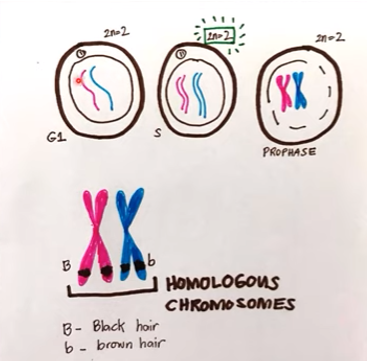
\includegraphics[scale=0.7]{G1SPDrawing.png}
\begin{itemize}
    \item G1 and S are both at 2n=2 despite the DNA being duplicated
    \item Chromosome number does not correspond to the DNA material, but to the DNA present in the material
    \item In Prophase the nuclear membrane starts to disentigrate and so does the centrosome as they go to the opposite pole
    \item As seen in the bottom figure the Locus can be seen as it is where the gene is locacted, it can be designated as \textit{B} - black hair, and \textit{b} - brown hair, so this cell is hetorogenous, but if they were both BB they were homozygous.
\end{itemize}
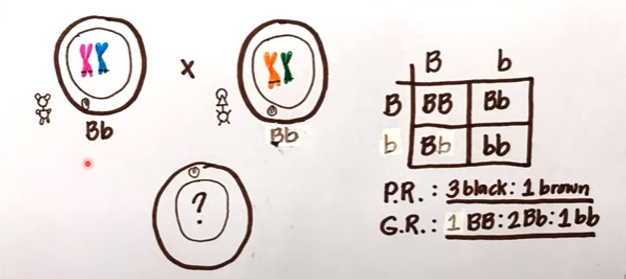
\includegraphics[scale=0.5]{BbBb.png}
\begin{itemize}
    \item As seen above where two hetorogenous pairs combine.
    \item Phenotypic Ratio: As long as there is one \textit{B} or dominant gene it would be automatically that property and not the subdominant one
\end{itemize}
Note: We actually have 23 different types of chromosomes, 1-22 are  the autosomes as they are somatic cells and express our characteristics, while the 23rd chromosome (XY) is responsible for representing our biological gender.
Difference between Genes and Alleles: Alleles are variations of specific genes. All of these combined is called the karyotype with all the Homologous pairs present. Additionally, the smaller the chromosome is less preferred or a newer gene. Human evolving is chromosomes getting shorter as there are some hormones that are no longer present.


Research how many centromeres are present.

\subsubsection*{Diploid vs Haploid}
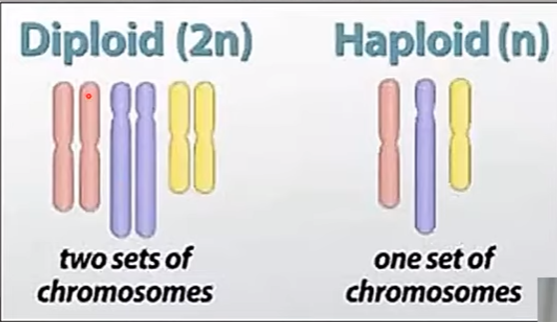
\includegraphics[scale=0.5]{DipVsHap.png}
\begin{itemize}
    \item Diploid: number is 2n with two representatives / homologues
    \item Haploid: Only one representative
    \item Mitosis needs Diploids while Meiosis needs Haploids, as when the  sperm cell and egg cell combines it needs to equal 46 or 23+23=46
    \item Figures explaining this can be seen below
\end{itemize}
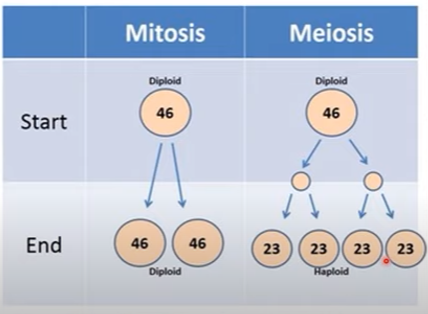
\includegraphics[scale=0.6]{MitMeoDipHap.png}


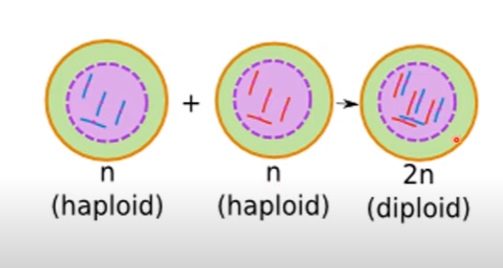
\includegraphics[scale=0.5]{nn2n.png}

\section*{Life Cycle of a Cell}
Note: please note that the majority of the cell's life cycle isn't  always dividing.

\includegraphics*[scale=0.8]{celllifecycle.png}

\subsubsection*{G1}
\begin{itemize}
    \item Where the cellular extents excluding the chromosomes extend, it is currently half of a cell and all of it's contents need to be duplicated
    \item centrosome: organelle which contains the centriole, where the spindle fibers will pertrude. centriole is duplicated here (only 1 in Gap 0, but 2 in Gap 1)
    \item The cell recovers, after duplication the cells grow and it fulfills its function. e.g. if you were a liver cell after division you would have your stuff replenishing while carrying out it's functions
\end{itemize}
\subsubsection*{S}
\begin{itemize}
    \item Stands for itemize, it is where the chromosomes are duplicated
    \item Still not condensed (chromatin)
    \item During the discussion in DNA replication, there are proteins involved in replicating the DNA and the checkpoint is there to make sure its okay. Protein initiated checkpoint, but the mechanism is different compared to the other phases.
\end{itemize}
\subsubsection*{G2}
\begin{itemize}
    \item Double checking of the chromosomes to see if they are ready for cell division
    \item centrioles start to separate and spindle fibers go to opposite poles
    \item 
\end{itemize}
Note: Some cells do not reproduce anymore and die, such as nerve cells.
\subsubsection*{G0}
\begin{itemize}
    \item After G1, where cell cycle arrest happens as it isn't dividing and isn't preparing to divide.
    \item Two Homologous chromatin pairs, 2n=4
    \item 
\end{itemize}
\subsubsection*{Apoptosis}
\begin{itemize}
    \item programmed cell death, used in early development (e.g. tadpoles not growing their tails anymore)
    \item can also be used to get rid of damaged cells beyond repair
\end{itemize}
\subsection*{Regulation of Cell Phases}
\subsubsection*{G1 Checkpoint}
\begin{itemize}
    \item Nutrients, Growth factors, DNA damage
\end{itemize}
\subsubsection*{G2  Checkpoint}
\begin{itemize}
    \item Cell size, DNA replication
\end{itemize}
\subsubsection*{Metaphase Checkpoint}
\begin{itemize}
    \item Chromosome spindle attachment
\end{itemize}
\subsection*{Use of cyclin dependent kinase}
\begin{itemize}
    \item activated when it is phosphorelated and a phosphate group attaches to the kinase to become  active
    \item helps the cell proceed to another phase
    \item Can be found in the cyclin (substrate), and the enzyme is the kinase
    \item G1: is almost always present
    \item G/S Cyclin: Spikes between G1 and S Phase to signify the S Phase transition
    \item S Cyclin: Raises in  the S phase and peaks at G2, and drops rapidly at the M Phase
    \item M cyclin: starts from S phase, rapidly shoots up between G2 and M phase peaking at the M phase and dropping down immediately.
\end{itemize}
\includegraphics*[scale=0.6]{cyclin.png}
\section*{Cell Division}
\subsection*{Interphase}

\includegraphics*[scale=0.5]{interphase.png}

\subsection*{Mitosis}
\begin{itemize}
    \item You can see the chromatin in the Interphase
\end{itemize}
\subsubsection*{Prophase}

\includegraphics*[scale=0.5]{prophase.png}


\begin{itemize}
    \item chromatin DNA starts to condense turning into DNA becomes a strand of chromatin
    \item nuclear membrane starts to disentigrate
\end{itemize}
\subsubsection*{Metaphase}


\includegraphics*[scale=0.5]{metaphase.png}


\begin{itemize}
    \item DNA materials is concentrated into the center / align to the middle
    \item spindle fibers conect to the Kinetochore
    \item In plant cells there are no centrosomes but a methaphase is used to separate them
\end{itemize}
\subsubsection*{Anaphase}


\includegraphics*[scale=0.5]{anaphase.png}


\begin{itemize}
    \item The chromosomes move to two opposite poles
    \item Becomes 2n=4 and 2n=4 as the chromatids are now split, and the candidates have increased
\end{itemize}
\subsubsection*{Telophase}


\includegraphics*[scale=0.45]{telophase.png}


\begin{itemize}
    \item Division  of the nuclear contents
\end{itemize}
\subsubsection*{Cytokinesis}
\begin{itemize}
    \item Division of the cytoplasmic conents (the space outside of the nucleus)
    \item movement of the cytoplasm
    \item where the cleavage furrow can be seen
\end{itemize}
\subsubsection*{Root Tip Cell Division Information}
\begin{itemize}
    \item Area of cell division: active cell division
    \item Area of elongation: no more cell division
    \item Area of maturation: cells are going to die in order to absorb water
\end{itemize}
\subsubsection*{Bacteria and mitosis}
Note: Bacteria does not go through cell division, but undergoes binary fission instead.
\subsection*{Meiosis}
\subsubsection*{Prophase 1}
Goal: condense the homologus pair to each other


Leptonema


\includegraphics*[scale=0.9]{leptonema.png}
\begin{itemize}
    \item duplicated chromatins are now condensed
    \item the condensing in the centromere increases
\end{itemize}
Zygonema


\includegraphics*[scale=0.9]{zygonema.png}
\begin{itemize}
    \item members of the homologous pairs get attached with one another
    \item synaptonemal complex
\end{itemize}
Pachynema


\includegraphics*[scale=0.9]{pachynema.png}
\begin{itemize}
    \item Complete attachment of the Homologous pairs
    \item The crossing over also happens here
\end{itemize}
Diplonema


\includegraphics*[scale=0.9]{diplonema.png}
\begin{itemize}
    \item Decongenstion
    \item Visible effects of crossing over
    \item Between two homologoues the average amount is 1-3 crossing overs
    \item Called chiasma, plural chiasmata
    \item these crossing overs are called tetral, bivalence
    \item centrioles are going farther and farther away from each other
\end{itemize}
Diakinesis


\includegraphics*[scale=0.9]{diakineses.png}
\begin{itemize}
    \item The nuclear membrane starts to disentigrate
    \item Centrioles are at the opposite sides
\end{itemize}
Metaphase I In Meiosis


\includegraphics*[scale=0.9]{mim.png}
\begin{itemize}
    \item the Homologous pairs align at the middle, not the sister chromatids
    \item This is because of the chiasma
\end{itemize}
Anaphase I In Meiosis


\includegraphics*[scale=0.9]{aim.png}
\begin{itemize}
    \item becomes n=2 and n=2
    \item two haploid cells
\end{itemize}
These are then split again, and become 4 cells with 4 haploids at n = 2 once it is at it's final form
\subsubsection*{Spermatogenesis and Oogenesis}
\begin{itemize}
    \item Spermatogenesis: creates more sperm cells
    \item Oogenesis: creates polar bodies instead of more egg cells
    \item Reason why there is more sperm cells than egg cells
\end{itemize}
\section*{Contributions to Genetic Variations}
\subsection*{Independent Assortment}


\includegraphics*[scale=0.45]{ia.png}
\begin{itemize}
    \item Given a homologus pair, one homologous pair's crossing over is independent of each other. It can cross over to its pair, and is not dependent to other chromosomes.
    \item Genes are independent of each other
    \item This independence causes a chain reaction the further it reproduces
\end{itemize} 

\subsection*{Crossing Over}


\includegraphics*[scale=0.45]{co.png}
\begin{itemize}
    \item We can often only think of it as one paternal and one maternal, but they can cross over
\end{itemize}

\subsection*{Random Fertilization}
\begin{itemize}
    \item Due to the genetic variations of sperm and egg cells, so we are very unique even to genetics
    \item Almost impossible to have the same genetics to a sibling
\end{itemize}
\section*{Note}
\includegraphics*[scale=0.3]{nilou.png}


Hi sir! Sorry if the layout is quite messy, as this is my first actual notes document on LaTeX, and I'm stil trying everything out. Hopefully by the next notes submission I could figure out a template and a structure to the notes instead of a bunch of bullet points. - Pope


Make sure to know how many parts are there in the chromosome per cell.
\end{document}
